The ATLAS  detector's data acquisition system, illustrated in Figure \ref{fig:tdaq_diagram}, makes use of a multi-tiered trigger to reduce the
bandwidth from the LHC proton bunch crossing rate of 40 MHz
to the 1 kHz written to disk \cite{evolution1,evolution2}. The first tier (Level-1 or L1) \cite{l1}, implemented in real time with custom electronics, 
makes an early event selection to determine if any objects of interest are present and reduces the data flow to 
100 kHz. The second tier, referred to as the High Level Trigger (HLT) \cite{hlt}, is implemented on a commodity computing cluster running custom triggering software. The HLT uses information from the
hardware based L1 system to guide the retrieval of information from the Readout System (ROS) \cite{ros}. 

\begin{figure}[!t]
\centering
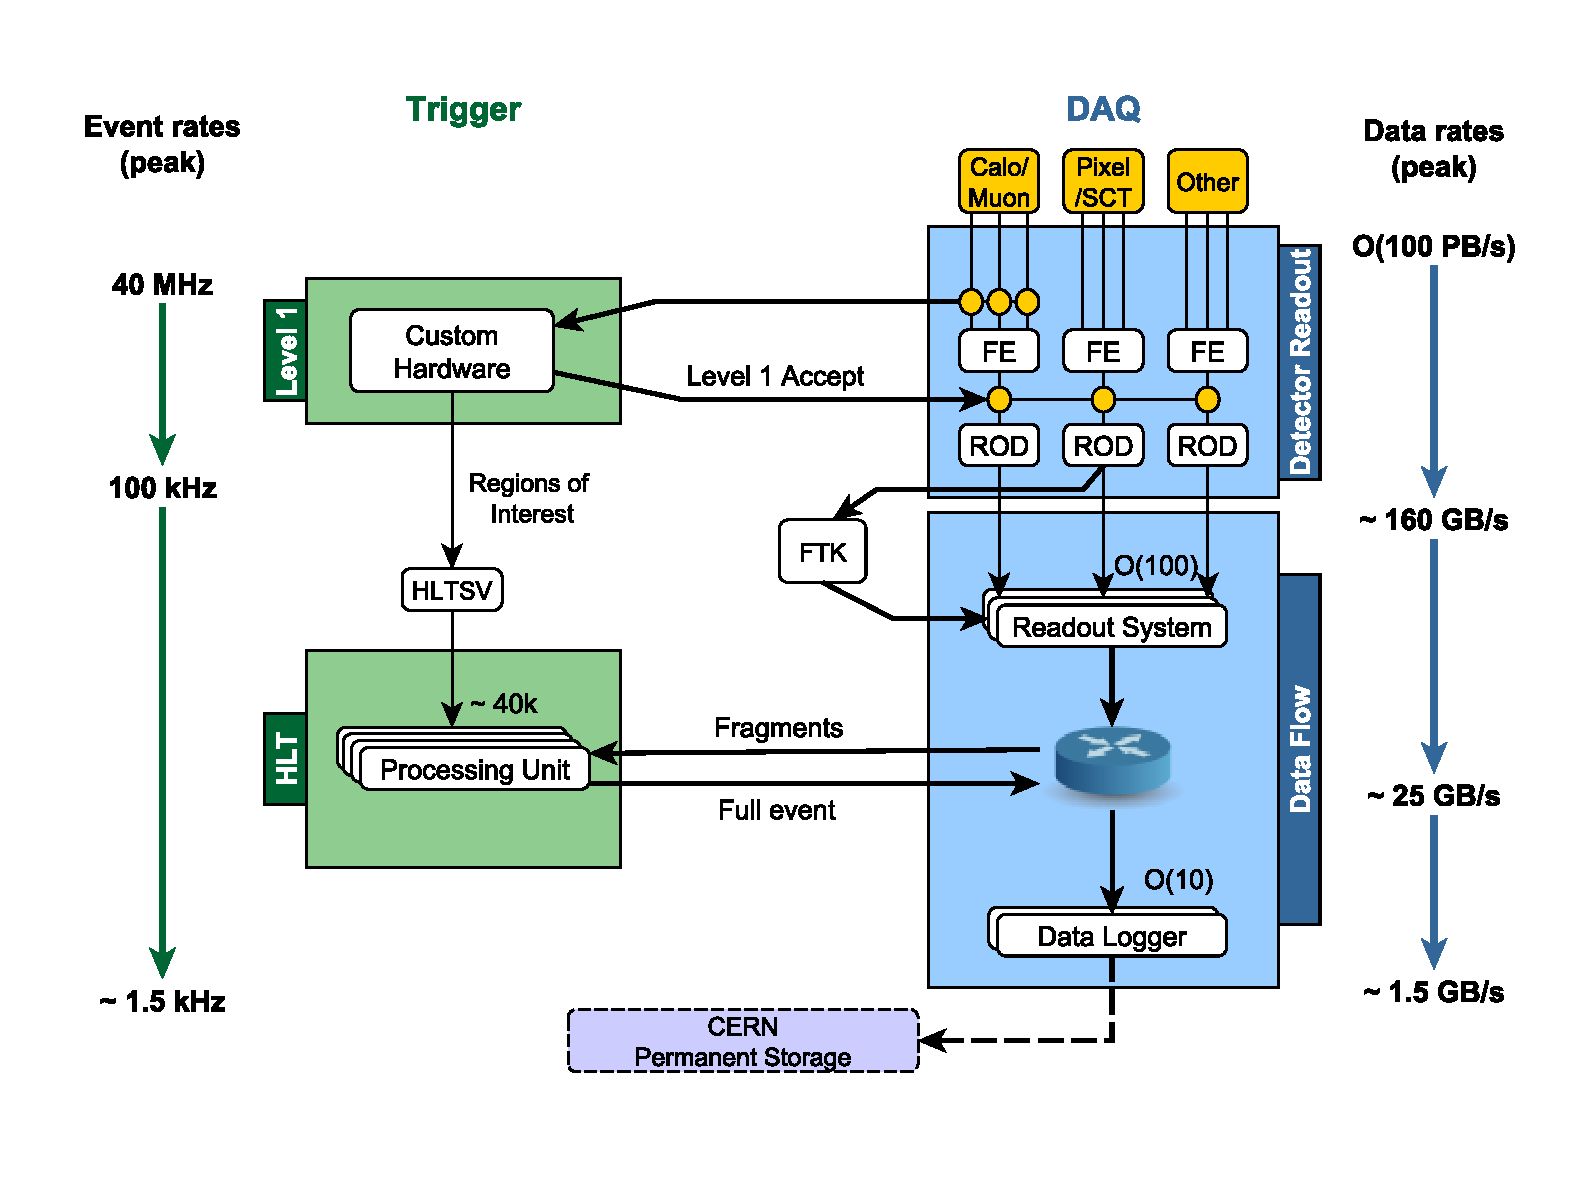
\includegraphics[width=1.\textwidth]{tdaqFullNew2016}
\vspace{-0.5cm}
\caption{ATLAS TDAQ architecture.}
\label{fig:tdaq_diagram}
\end{figure} 

\subsection{Hardware Trigger (L1)}
The L1 trigger has access to raw data from the calorimeters and the 
muon system. The L1 calorimeter trigger (L1Calo) uses reduced-granularity
information from 7200 trigger towers of the calorimeters. These trigger 
towers are divided in a $\Delta\eta\times\Delta\phi$ space by 
$0.1 \times 0.1$ over most of the calorimeter, and larger in the forward 
region. A decision is made based on the multiplicities and $E_{\rm{T}}$ 
thresholds of the objects 
identified by the L1Calo algorithms: electromagnetic (EM) clusters, 
$\tau$-leptons, jets, missing transverse energy, scalar sum $E_{\rm{T}}$, 
and total transverse energy of the L1 jets.
The L1 muon trigger (L1muon) uses measurements of the trajectories of muons 
in the RPC and TGC trigger chambers, located in the barrel and end-cap regions 
of the muon spectrometer. The multiplicity of the various muon \pt thresholds
is input to the trigger decision.

The central trigger processor (CTP) combines results from the L1Muon and L1Calo
triggers to issue an overall L1 accept or reject decision.
To facilitate this task, the CTP programs up to 256 configurations that 
consist of various combinations of $E_{\rm{T}}$ and \pt requirements, 
or thresholds.
The CTP has the capability of implementing different isolation criteria 
to the different objects such as the L1 EM clusters. 
A trigger menu is implemented as a collection of L1 items, each containing a 
logical combination of one or more configured L1 thresholds. 
For example, the item L1\_EM30i refers to an event requiring at least one 
isolated EM object with a transverse energy of $E_{\rm{T}} > 30$ \GeV. 
If the rates of a particular 
object is high, such as EM objects with low momentum, a prescale factor $\alpha$ is applied to the L1 item in the menu, where only 1 in $\alpha$
events is passed to the HLT. The L1 prescales are generally adjusted to 
maintain the optimal use of the allocated bandwidth for an L1 item during 
data-taking since the luminosity drops over the course of a run.

The L1 trigger has a 2.5 $\mu$s latency where the data fragments are 
held in pipeline buffers located within detector-specific front-end 
electronics. 
Once the CTP issues an accept, the data is pushed to detector-specific 
Readout Drivers (RODs), then transferred to the Readout System (ROS). 
The rest of the chain is described next. 

\begin{figure}[t!]
\centering
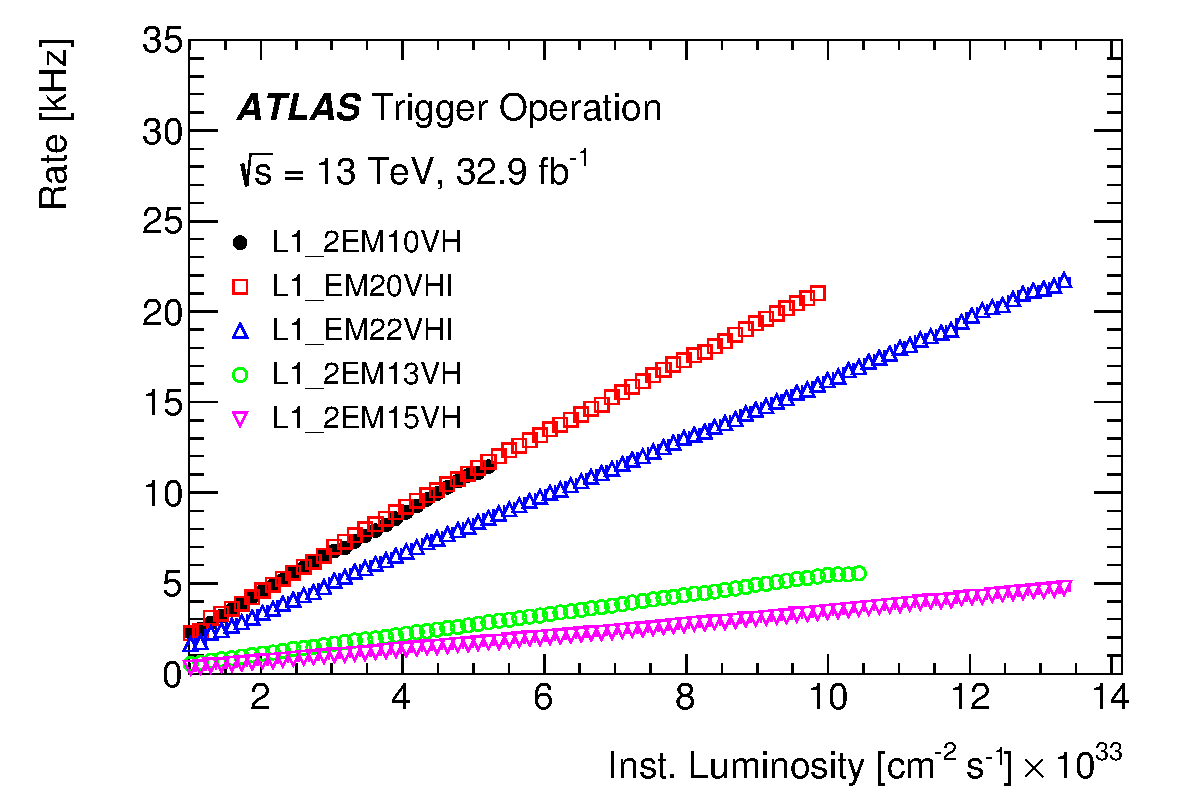
\includegraphics[width=0.95\textwidth]{L1_EM_Full2016}
\caption{Output rates of Level-1 EM triggers as a function of the uncalibrated instantaneous luminosity measured online during the 2016 proton-proton data taking at a center-of-mass energy of 13 TeV.
Rates are shown only for unprescaled triggers. All trigger rates show a linear dependency with instantaneous luminosity.}
\label{fig:}
\end{figure} 




\subsection{Dataflow Challenges in Run-2}
The function of the DAQ system is to efficiently buffer, transport, and record the events that were selected by the trigger system. 
Its performance is affected by the instantaneous luminosity that leads to busy events with multiple proton-proton interactions occurring in each 
bunch crossing, referred to as pileup. The high pileup results in a higher data volume collected by the detector that needs to be 
processed at the required rate to avoid exerting back-pressure on the L1 system. 
In Run 2, the LHC has exceeded the designed instantaneous luminosity of \\$10^{34}$ cm$^{-2}$ s$^{-1}$ leading to pileup of~ $<\mu>=30$ or more as shown 
in Figures \ref{fig:exp.lhc.peakLumiByFill} and \ref{fig:exp.mu_2015_2016}.
%% \begin{figure}[t!]
%% \centering
%% \begin{subfigure}[t]{0.48\textwidth}
%% 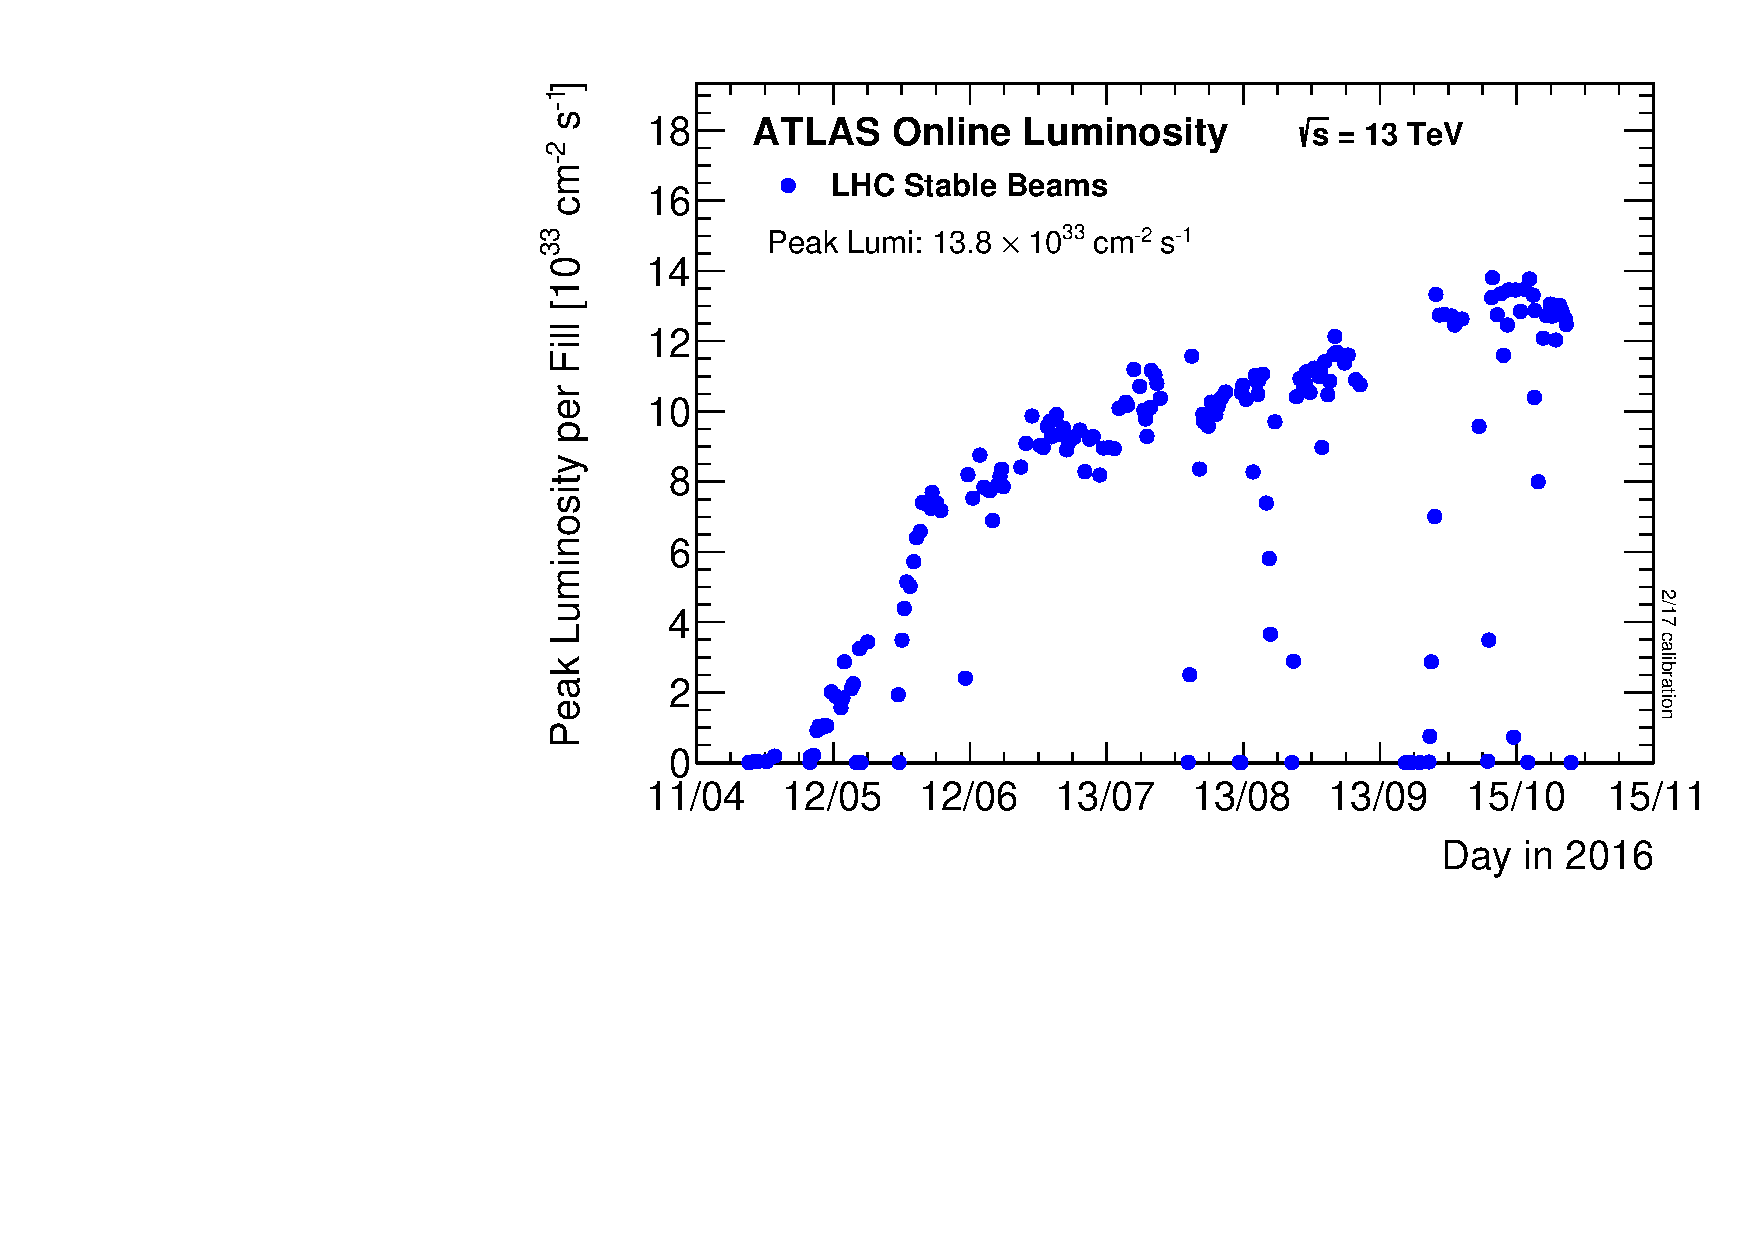
\includegraphics[width=\textwidth]{peakLumiByFill}
%% \end{subfigure}
%% \begin{subfigure}[t]{0.48\textwidth}
%% 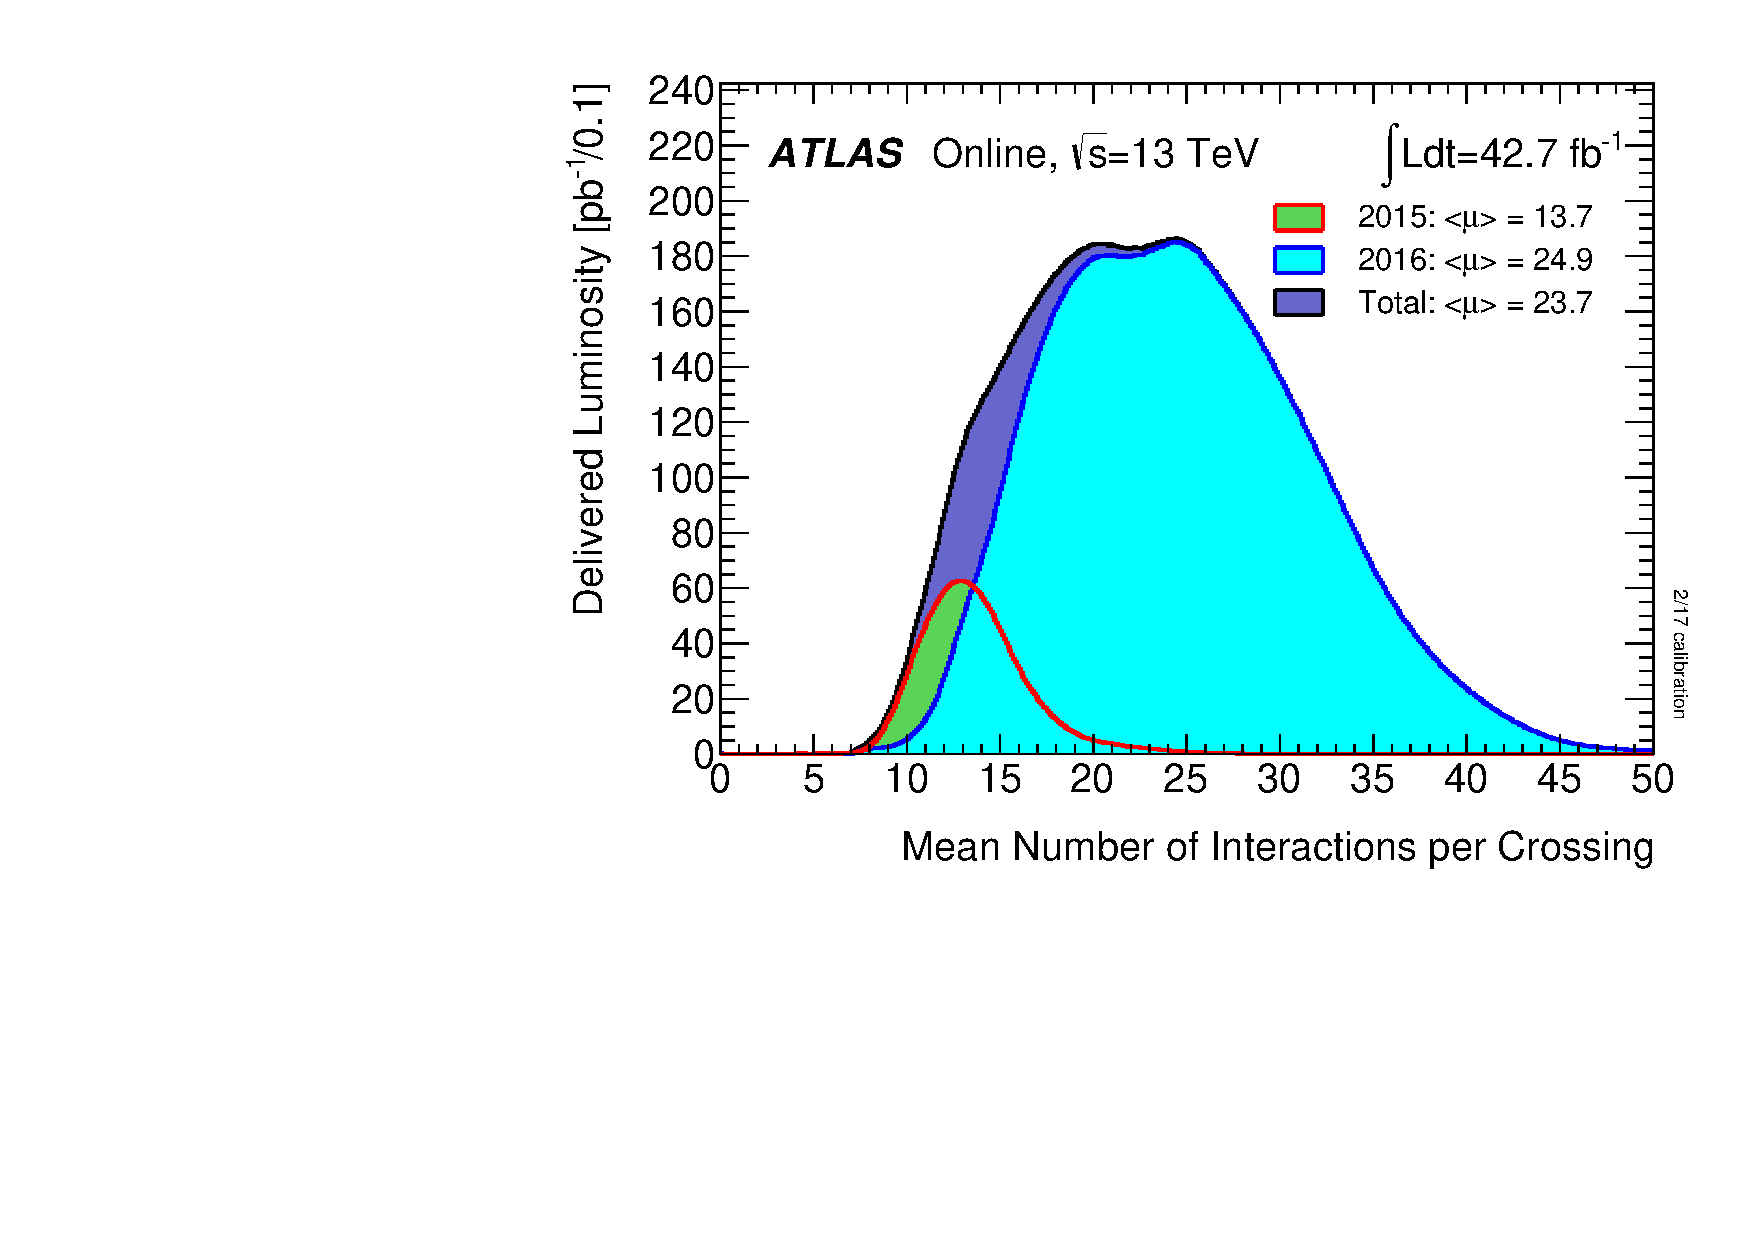
\includegraphics[width=\textwidth]{mu_2015_2016}
%% \end{subfigure}
%% %\vspace{-2cm}
%% \caption{Run conditions during Run 2: ATLAS peak online luminosity per fill (left), ATLAS online pileup (right) \cite{atlasTwiki}.}
%% \label{fig:lumi_pileup_1}
%% \end{figure} 
The L1 accept 
rate has also increased from 75 kHz in Run 1 to 100 kHz in Run 2 and the average output rate of the data logger system has 
increased from 400-600 Hz in Run 1 to about 3 kHz with 1.5 kHz for physics data. 
Moreover, there were new detectors that were added in Run 2
(Insertable B-layer (IBL), L1 topological trigger, Fast Tracker (FTK))\cite{Aad:1602235} leading to 
an increase of 20\% in the number of readout channels. 
To cope with these changes, the ATLAS TDAQ system was upgraded during Run-2
simplifying its architecture and increasing its flexibility.
To be able to deliver more rate to the High Level Trigger (HLT), the upgrade also targeted the Readout System (ROS)\cite{PanduroVazquez2016939}. 
For the same reason the two levels of the HLT system were collapsed into a single level which made the system more flexible 
 allowing for incremental data retrieval and analysis. 
The dataflow network system was re-designed to increase its capacity and simplify its architecture\cite{1742-6596-396-1-012033}.

\subsection{ATLAS Dataflow Design}

In Run 1, the computing farm was subdivided into several slices, with 
each slice managed by a dedicated supervisor. This layout has been 
dropped in favor of global management by a single farm master 
operating at 100 kHz referred to as the HLT supervisor (HLTSV). 
The Region of Interest Builder (RoIB) that assembles the RoIs
previously implemented on a VMEbus 
system is now integrated with the HLTSV and the RoI building done in software.
Chapter~\ref{chap:roib} is dedicated to the work of the author in the RoIB evolution. 
The change in the HLT architecture from two to one level
required re-writing the HLT software and algorithms in such a way that 
each computing node in the farm can perform all processing steps. The handling of these
processing steps is done by a single Data Collection Manager (DCM) process 
running on each HLT node to manage the L1 RoIs, the dataflow 
between the ROS and the HLT processing units (HLTPU), 
the event building processes, and the data logging.
 In the new architecture, the computing resources are managed more efficiently
by balancing the utilization of all cluster nodes depending on the active HLT 
algorithms and by sharing the HLT code and services to reduce memory and 
resource usage. 

The dataflow network shown in Figure~\ref{fig:net_diagram} was simplified and upgraded to handle a larger data volume.
A single network is used for 
RoI based access from the ROS, event 
building in the HLT processing nodes, and sending data for logging. 
A 10 GbE connectivity has been adopted throughout  the dataflow system
resulting in a factor of four increase in bandwidth between the data loggers and
the permanent storage, and a 4$\times$10 GbE output from each ROS PC to the core routers. 
The HLTSV and the HLT racks are all connected directly to each of the two core routers via 
 2$\times$10 GbE connections. Each HLT rack is hosting up to 40 nodes connected by 2$\times$1 GbE to the top-rack switches. 
The capacity of the routers can accommodate
an increase in the number of HLT server racks and ROS PCs by a factor of two, 
which will be needed when the system scales as run conditions 
change. The core routers also provide load balancing and traffic shaping protocols \cite{1742-6596-396-1-012033}
to distribute the data throughout the system more evenly. A duplication of core routers provide link redundancy at every level in 
case of link or switch failures.


\begin{figure}[t!]
\centering
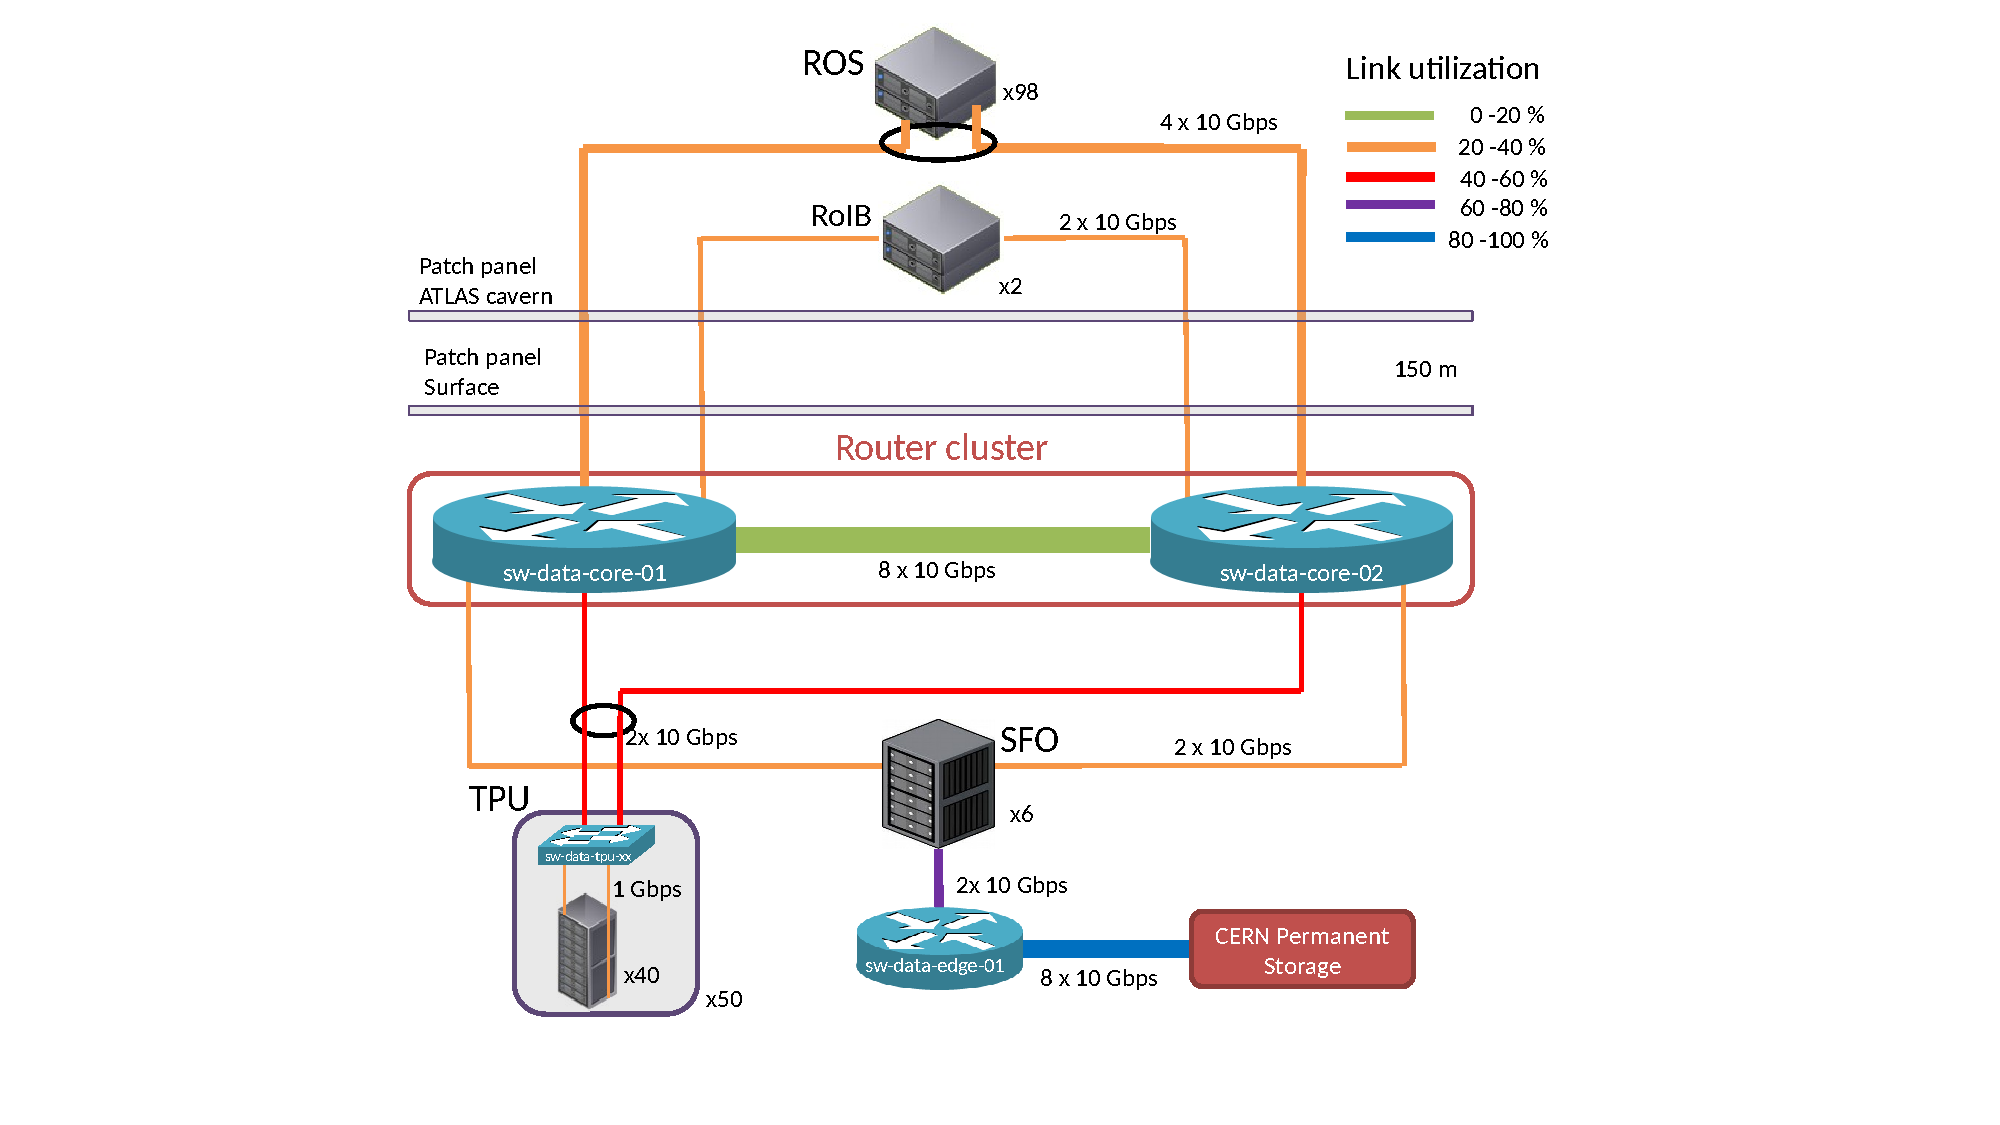
\includegraphics[width=1.2\textwidth]{network} 
%\vspace{-1cm}
\caption{ATLAS Dataflow network}
\label{fig:net_diagram}
\end{figure} 

To take advantage of multi-core architectures, the dataflow
 software is using multi-threaded software design for CPU consuming operations.
The Input/Output of the dataflow is based on asynchronous communication using industry standard libraries
such as the Boost::ASIO library. All the ATLAS software suite was switched to exclusively 64 bit operation in 2016.



In summary, the elements of the Run-2 ATLAS dataflow are:

\begin{itemize}
\item The Readout Sytem (ROS) buffers front-end data from the detectors and provides a standard interface to the DAQ system.
\item The Region of Interest Builder (RoIB) receives the L1 trigger information from the RoIs and combines the information for the HLT supervisor.
\item The HLT Supervisor (HLTSV) can handle the input from the RoIB and manage the HLT computing farm of about 2000 machines at 
over 100 kHz.
\item The Data Collection Manager (DCM) handles all Input/Output on the HLT nodes, including RoI requests from the HLT and full event building.
\item The HLT processing units (HLTPU) run the actual HLT algorithms which 
are forked from a single mother process to maximize memory sharing.
\item The Data loggers or SubFarm Output (SFO) are responsible for saving the 
accepted events to disk, and sending the files to CERN permanent storage infrastructure.
\end{itemize}



